\documentclass[twoside,a4paper,11pt,addpoints,answers]{exam}%answers,



\title{XX 1}
\date{}
\author{Juliette Fenogli}


\usepackage{siunitx}
\usepackage{mystyles}
\usepackage[export]{adjustbox}
\usepackage{mathpazo}
\usepackage{booktabs}
\usepackage{framed}
\usepackage{mdframed}
\usepackage[most]{tcolorbox}
\usepackage{listings}
\usepackage{mhchem}
\usepackage{tcolorbox}

\usepackage{subfig}
\usepackage{float}

\lstset
{upquote=true,
columns=flexible,
    basicstyle=\small\tt\hbox{}, 
	basicstyle=\ttfamily,
	language=Python,
    framesep=\fboxsep,
    framerule=\fboxrule,
    xleftmargin=\dimexpr\fboxsep+\fboxrule,
    xrightmargin=\dimexpr\fboxsep+\fboxrule,
	commentstyle=\color{gray},
	frame=single,
	rulecolor=\color{green!5},
	backgroundcolor=\color{gray!5},
	breaklines,
	numbers=left, 
	numbersep=5pt,  
	numberstyle=\scriptsize \ttfamily\color{gray},
	breakindent=1.5em,
	literate={Δ}{{$\mathtt{\Delta}$}}1 {‡}{{$\mathtt{\ddagger}$}}1
  {á}{{\'a}}1 {é}{{\'e}}1 {í}{{\'i}}1 {ó}{{\'o}}1 {ú}{{\'u}}1
  {Á}{{\'A}}1 {É}{{\'E}}1 {Í}{{\'I}}1 {Ó}{{\'O}}1 {Ú}{{\'U}}1
  {à}{{\`a~}}1 {è}{{\`e}}1 {ì}{{\`i}}1 {ò}{{\`o}}1 {ù}{{\`u}}1
  {À}{{\`A~}}1 {È}{{\'E}}1 {Ì}{{\`I}}1 {Ò}{{\`O}}1 {Ù}{{\`U}}1
  {ä}{{\"a}}1 {ë}{{\"e}}1 {ï}{{\"i}}1 {ö}{{\"o}}1 {ü}{{\"u}}1
  {Ä}{{\"A}}1 {Ë}{{\"E}}1 {Ï}{{\"I}}1 {Ö}{{\"O}}1 {Ü}{{\"U}}1
  {â}{{\^a}}1 {ê}{{\^e}}1 {î}{{\^i}}1 {ô}{{\^o}}1 {û}{{\^u}}1
  {Â}{{\^A}}1 {Ê}{{\^E}}1 {Î}{{\^I}}1 {Ô}{{\^O}}1 {Û}{{\^U}}1
  {œ}{{\oe}}1 {Œ}{{\OE}}1 {æ}{{\ae}}1 {Æ}{{\AE}}1 {ß}{{\ss}}1
  {ç}{{\c c}}1 {Ç}{{\c C}}1 {ø}{{\o}}1 {å}{{\r a}}1 {Å}{{\r A}}1
  {€}{{\EUR}}1 {£}{{\pounds}}1 {×}{{$\times$}}1,       
}


\usepackage{adjustbox}
\usepackage{colortbl}
\usepackage{fontawesome}
\usepackage{todonotes}
\usepackage{listings} %codes python
\usepackage{parskip}

\usepackage{subfig}


%Columns Spacing
\newcolumntype{C}[1]{>{\centering\let\newline\\\arraybackslash\hspace{0pt}}m{#1}}
\newcolumntype{M}[1]{>{\centering\arraybackslash}m{#1}}

%Colorbox
\newtcolorbox{mybox}{colback=white!5!white,
colframe=black!75!black,left=7mm}

\newcounter{foo} %Counter questions

\begin{document}

\begin{minipage}{0.33\textwidth}
Noms-Prénoms du binôme
\end{minipage}\begin{minipage}{0.33\textwidth}
$n^\circ 1$ :
\end{minipage}\begin{minipage}{0.33\textwidth}
$n^\circ 2$ :
\end{minipage}



\tito{Assemblage et montage d'une cellule solaire à colorant}

\paragraph*{But} 
Au cours de cette séance de TP, vous réaliserez la formulation d'une électrode à base de dioxyde de titane (\ce{TiO2}) et d'un verre conducteur à base d'oxyde d'indium et d'étain (ITO), deux composants essentiels des cellules solaires à colorant.

%à construire et utiliser des diagrammes binaires. Ceux-ci sont nécessaires à l'interprétation du comportement thermique ou de l'histoire thermique de mélanges solides. De plus, lors de la formation de l'alliage \ce{Pb}-\ce{Sn}, vous utiliserez un four particulier, appelé four tubulaire dont nous discuterons les avantages par rapport au four à moufle.

\begin{comment}
\paragraph*{Quelques remarques :}
\begin{enumerate}
\item {\color{red} Lors de ces deux séances de TP, il est attendu que vous teniez un cahier de laboratoire : observations, matériel, conditions opératoires doivent être référencées pour permettre le suivi de votre travail.}
\item Toute figure doit comporter des axes, des unités, un titre et des légendes. Le titre doit permettre à l'enseignant de comprendre l'essentiel de la figure sans avoir à lire le texte associé.
\item Toute donnée expérimentale doit être accompagnée des conditions expérimentales et outils associés à la mesure.
\end{enumerate}
\end{comment}

\paragraph*{Notations :}
On notera par $X^\star$ une espèce chimique $X$ photoexcitée.

\tableofcontents

\section{Mesures électrochimiques des performances de la photodiode}

\subsection{Dispositif de mesure}

Afin de faire l'acquisition des performances électrochimiques de la photodiode, nous allons réaliser des mesures sur un banc optique Metrohm couplé à un potentiostat-galvanostat, comme illustré à la Fig. \ref{fig:02}.

\begin{center}
\begin{minipage}{0.48\textwidth}
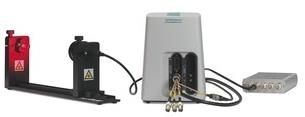
\includegraphics[width=\textwidth]{figures/Fig02}
\end{minipage}\begin{minipage}{0.48\textwidth}
\captionof{figure}{Banc optique Methohm Autolab. Le rail est équipé d'une LED rouge à \SI{627}{\nano\meter} à une distance de \SI{20}{\centi\meter} d'une photodiode de surface \SI{0.13}{\centi\meter\squared}}
\label{fig:02}
\end{minipage}
\end{center}

Un rail optique comporte des sources lumineuses quasi-monochromatiques de longueurs d'ondes : rouge $627 ~ \si{\nano\meter}$, bleue $470 ~ \si{\nano\meter}$ et une source monochromatique de lumière blanche reproduisant un corps noir de température \SI{4100}{\kelvin} à une intensité lumineuse de \SI{690}{\lumen}.

La source lumineuse est soumise à un courant $I$ modulable par le biais de galvonostat permettant de contrôler l'intensité lumineuse émise par la source. Le photorecepteur, de surface \SI{0.13}{\centi\meter\squared} est placé à une distance de \SI{20}{\centi\meter} de la source lumineuse. Toute mesure nécessite au préalable un étalonnage de la source lumineuse permettant de connaître la relation entre le courant appliqué et l'intensité lumineuse.

Afin de mesurer la caractéristique de la photodiode, le potentiostat se comporte comme une résistance variable, appelée charge, permettant de remonter à la caractéristique de la cellule.

\begin{comment}
\begin{questions}

\setcounter{question}{\thefoo}

\question[1] Identifier le rôle électrique joué par la photodiode dans le montage potentiostat-galvanostat/photodiode.

\begin{mybox}
\begin{solution}[5cm]

La photodiode reçoit de la lumière et convertit cette énergie en un courant électrique. Il en résulte que la photodiode joue le rôle de générateur électrique.
\end{solution}
\end{mybox}

Le potentiostat-galvostat joue le rôle analogue à un circuit composé d'une résistance variable, d'un voltmètre et d'un ampèremètre.

\question[3] Proposer un montage électrique simple permettant de faire l'acquisition de la caractéristique. Vous illustrerez le fonctionnement de ce circuit en vous appuyant sur les caractéristiques de la photodiode, illustrée à la Fig.\ref{fig:03} et celle des autres dipôles du circuit.

\begin{mybox}
\begin{solution}[5cm]

\textbf{Montages} [\textbf{2.0}] On peut proposer un montage courte ou longue dérivation permettant de récupérer le courant et la tension dans le circuit.

\begin{center}
\begin{minipage}{0.48\textwidth}
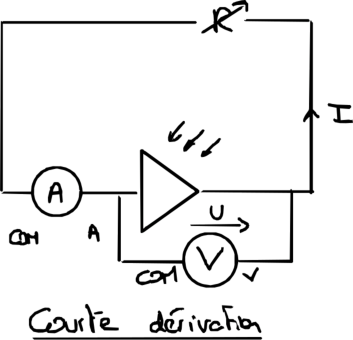
\includegraphics[width=0.9\textwidth]{figures/Corr01a}
\end{minipage}\begin{minipage}{0.48\textwidth}
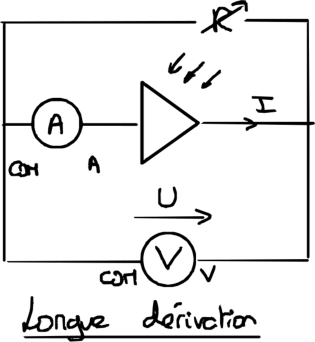
\includegraphics[width=0.9\textwidth]{figures/Corr01b}
\end{minipage}
\end{center}

\textbf{Echantillonage} [\textbf{1.0}] Dans le montage ci-dessus, la résistance joue le rôle de récepteur électrique et la photopile de générateur. En changeant la valeur de résistance, on fait l'acquisition de la caractéristique de la photopile. 

\begin{center}

\includegraphics[width=0.4\textwidth]{figures/Corr02}
\end{center}

\end{solution}
\end{mybox}


\setcounter{foo}{\value{question}}

\end{questions}
\end{comment}

\subsection{\'{E}talonnage de la source lumineuse}

Le dispositif expérimental est le même que décrit à la section précédente.

L'étalonnage de la source lumineuse va permettre d'identifier les courants à imposer au niveau de DEL (source lumineuse) pour obtenir une intensité lumineuse donnée.

\begin{figure}[H]
\begin{center}
\subfloat[\label{fig:TP2-01a}]{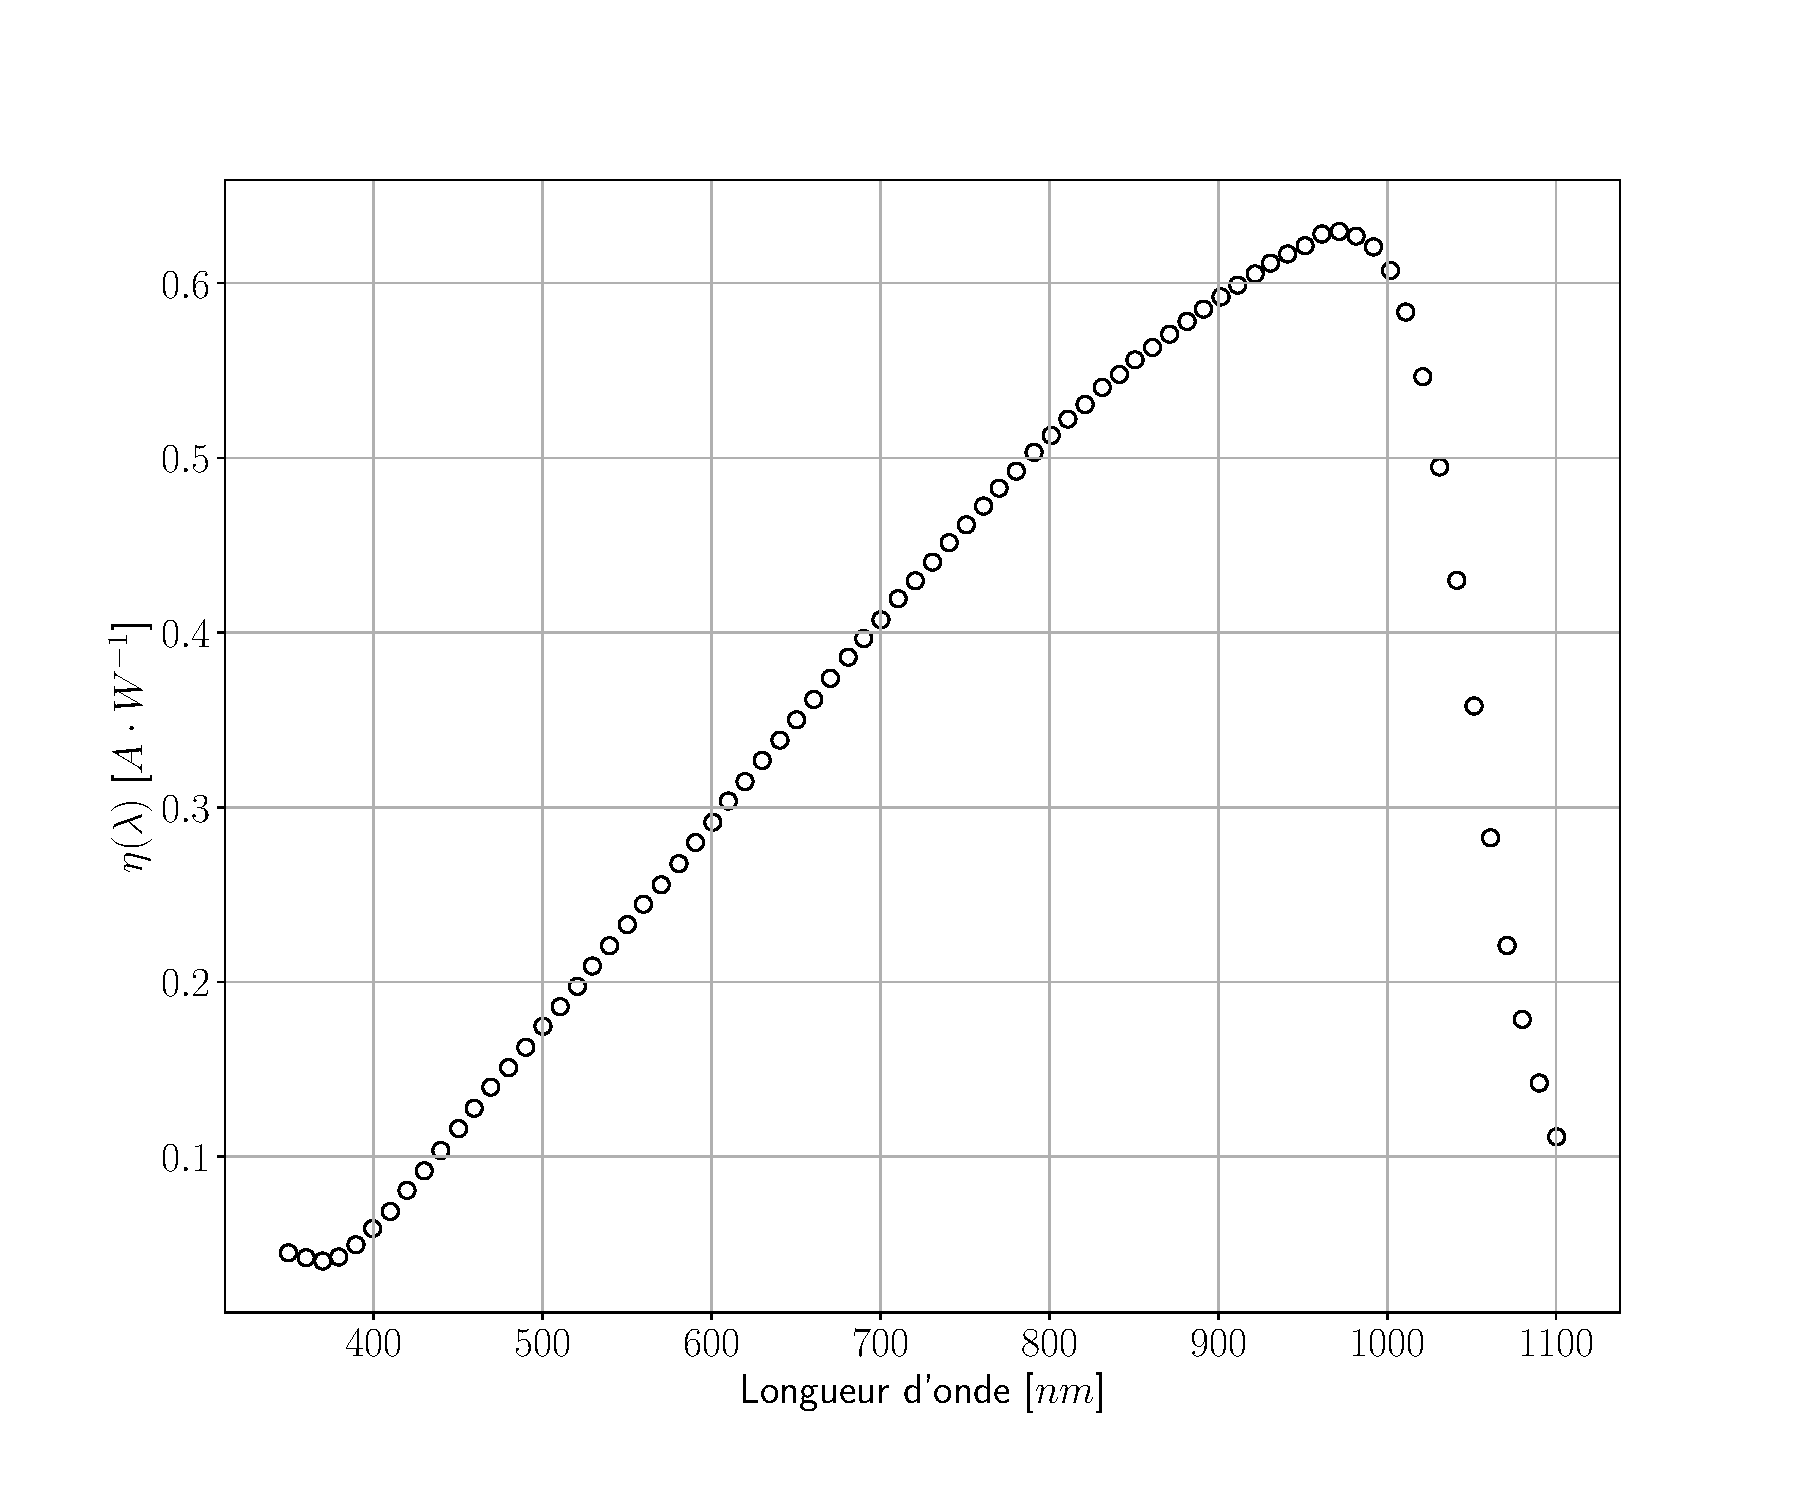
\includegraphics[width=0.48\textwidth]{figures/Fig01a}}\subfloat[\label{fig:TP2-01b}]{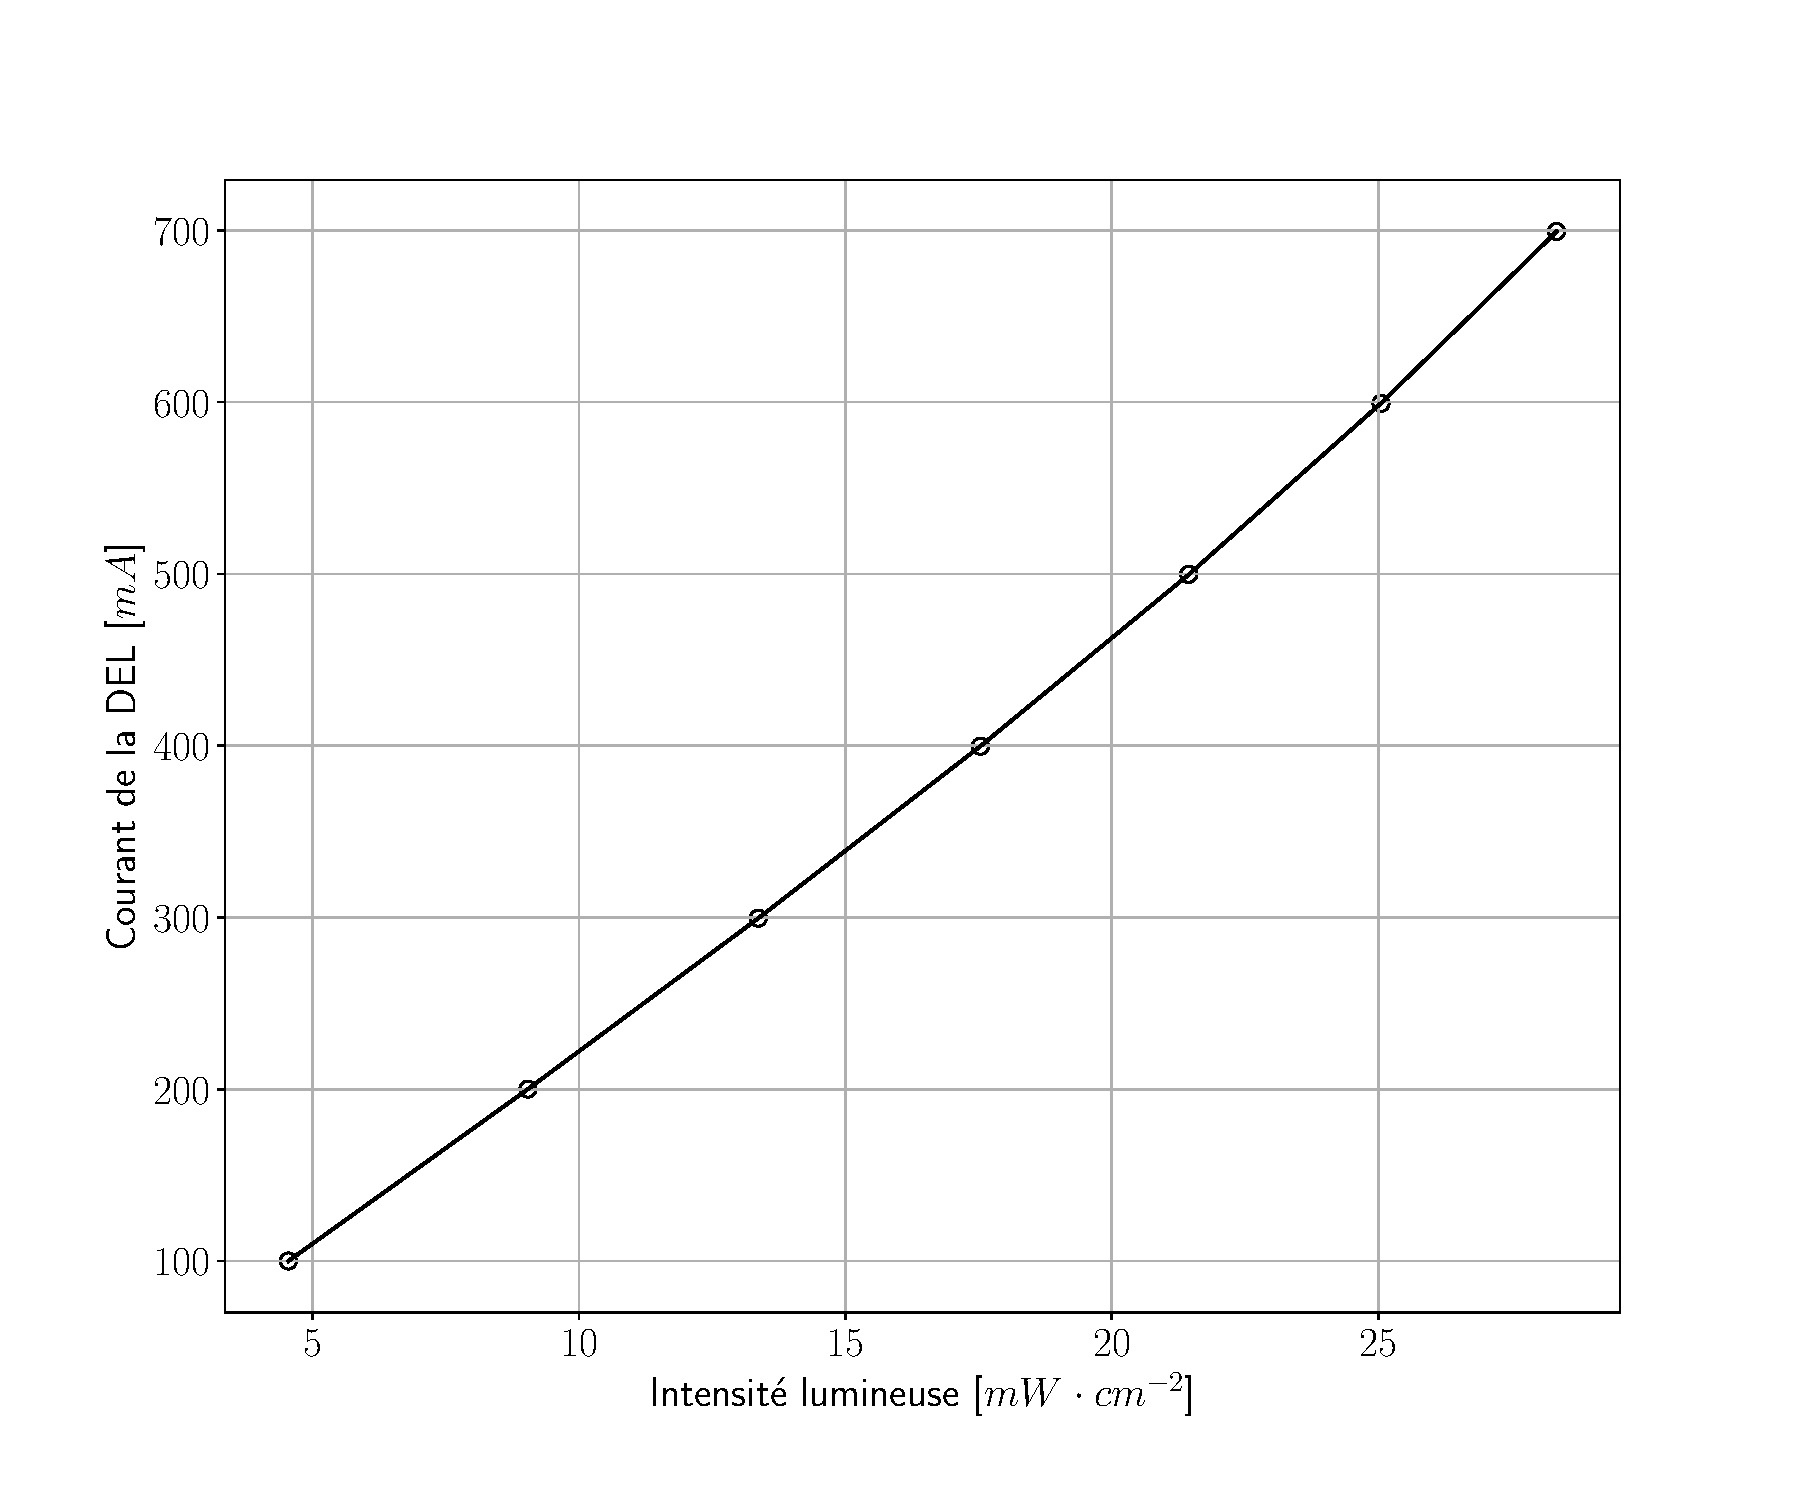
\includegraphics[width=0.48\textwidth]{figures/Fig01b}}
\end{center}
\caption{\ref{fig:TP2-01a} Evolution de la sensibilité en fonction de la longueur d'onde ; \ref{fig:TP2-01b} Courant de la diode électroluminescente en fonction de l'intensité lumineuse émise à \SI{627}{\nano\meter}}
\end{figure}

La DEL a été calibrée au préalable sur une source monochromatique à \SI{627}{\nano\meter} comme illustrée à la Fig.\ref{fig:TP2-01b}. \`{A} cette longueur d'onde, la relation entre intensité lumineuse et courant reçu a été modélisé à l'aide d'un polynôme d'ordre $4$.

\begin{center}
\begin{minipage}{0.5\textwidth}
\begin{align*}
I_{DEL} (P_{inc}) = a_0 + a_1 P_{inc} + a_2 P_{inc}^2 + a_3 P_{inc}^3 + a_4 P_{inc}^4
\end{align*}
\end{minipage}\begin{minipage}{0.5\textwidth}
\begin{tabular}{ccc}
\toprule
Paramètres & Unité & Valeur \\
\midrule
$a_0$ & \si{\milli\ampere} & $2.301$\\
$a_1$ & \si{\milli\ampere\centi\meter\squared\per\milli\watt} & $21.04$\\
$a_2$ & \si{\milli\ampere\centi\meter\tothe{4}\per\milli\watt\squared} & $11.62 \cdot 10^{-2}$ \\
$a_3$ & \si{\milli\ampere\centi\meter\tothe{6}\milli\watt\tothe{-3}} & $-40.48 \cdot 10^{-4}$ \\
$a_4$ & \si{\milli\ampere\centi\meter\tothe{8}\milli\watt\tothe{-4}} & $1.537 \cdot 10^{-4}$ \\
\bottomrule
\end{tabular}
\end{minipage}
\end{center}

Afin de connaître le comportement en longueur d'onde, le commercial fournit pour chaque photodiode étalon l'évolution de la sensibilité. La sensibilité, fonction de la longueur d'onde et notée $\eta (\lambda)$, correspond à la grandeur : 
\begin{align*}
\eta (\lambda) = \frac{\text{Courant généré par la photodiode}}{\text{Puissance de la lumière incidente}} \quad [\si{\ampere\per\watt}]
\end{align*}


\begin{comment}
\begin{questions}

\setcounter{question}{\thefoo}
\question[1\half] Calculer les courants à appliquer sur la DEL à \SI{627}{\nano\meter} pour avoir des intensités lumineuses de $0$, $5$, $10$, $15$, $20$ et \SI{25}{\milli\watt\per\centi\meter\squared}.

\begin{mybox}
\begin{solution}[5cm]

\begin{center}
\begin{tabular}{ccccccc}
\toprule
$P_{inc} ~ [\si{\milli\watt\per\centi\meter\squared}]$ & $0$ & $5$ & $10$ & $15$ & $20$ & $25$ \\
\midrule
$I(627 ~ \si{\nano\meter}) ~ [\si{\milli\ampere}]$ & $2.301$ & $110.0$ & $221.8$ & $338.2$ & $461.8$ & $597.7$ \\
\bottomrule
\end{tabular}
\end{center}

\end{solution}
\end{mybox}

\question[3\half] {\color{red} On souhaite avoir la même réponse en intensité de la photodiode à \SI{470}{\nano\meter} et \SI{627}{\nano\meter}. Calculer l'intensité incidente nécessaire à la nouvelle longueur d'onde. Que manque-il comme information pour pouvoir appliquer de telles puissances ?}
%{\color{red} En déduire les intensités lumineuses que l'on émettra avec la DEL à \SI{470}{\nano\meter}.}
\begin{mybox}
\begin{solution}[5cm]

Pour avoir une réponse constante de la photodiode, en posant $\lambda_1 = 627 ~ \si{\nano\meter}$ et $\lambda_2 = 470 ~ \si{\nano\meter}$, on peut écrire : [\textbf{0.5}]
\begin{align*}
I_{photodiode}^1 = I_{photodiode}^2
\end{align*}

On a alors : [\textbf{1.0}]
\begin{align*}
\eta ( \lambda_1 ) P_{inc}^1 = \eta ( \lambda_2 ) P_{inc}^2 &\iff \eta ( \lambda_1 ) P_{inc}^1 = \eta ( \lambda_2 ) P_{inc}^2 \\
P_{inc}^2 = \frac{\eta ( \lambda_1 )}{\eta ( \lambda_2 )} P_{inc}^1
\end{align*}

La courbe de \ref{fig:TP2-01a} nous permet de remonter aux valeurs de sensibilité aux longueurs d'onde $\lambda_1$ et $\lambda_2$ : [\textbf{0.5}]
\begin{align*}
\eta ( \lambda_1 ) &= 0.325 ~ \si{\ampere\per\watt} \\
\eta ( \lambda_2 ) &= 0.140 ~ \si{\ampere\per\watt}
\end{align*}

\textbf{AN :} [\textbf{1.0}]

\begin{center}
\begin{tabular}{ccccccc}
\toprule
$P_{inc}^1 ~ [\si{\watt\per\centi\meter\squared}]$ & $0$ & $5$ & $10$  & $15$ & $20$ & $25$ \\
\midrule
$P_{inc}^2 ~ [\si{\watt\per\centi\meter\squared}]$ & $0$ & $11.6$ & $23.2$ & $34.8$ & $46.4$ & $58.0$ \\
\bottomrule
\end{tabular}
\end{center}

~\

\textbf{Conversion puissance-courant} Pour faire la conversion puissance, courant, il faudrait éavoir préalablement étalonnée la diodeelectroluminescente à \SI{470}{\nano\meter}. [\textbf{0.5}]



\end{solution}
\end{mybox}

\setcounter{foo}{\thequestion}
\end{questions}
\end{comment}

\subsection{Exploiter une caractéristique de photodiode}

La caractéristique de la photodiode est caractérisée par un certains nombre de paramètres : 

\begin{itemize}
\item \textbf{OCV (ou OCP) : Open-Circuit Voltage} La tension à courant nul est la tension aux bornes de la photodiode branchée à un récepteur de résistance infinie, c'est-à-dire pour un courant nul dans le circuit.
\item \textbf{OCC : Open-Circuit Current} Le courant de court-circuit est le courant produit par la photodiode branchée à un récepteur parfait de résistance nulle.
\end{itemize}

Comme illustrée à la Fig.\ref{fig:03}, un point important est le point $\bullet = (U_{max}, I_{max})$ correspondant aux conditions de tension et courant permettant d'obtenir une puissance électrique cédée maximale : 
\begin{align*}
P_{max} = I_{max} \cdot U_{max}
\end{align*}

De ces propriétés électriques, un expérimentateur peut calculer le facteur de forme, grandeur sans unité, noté $FF$ dont la valeur est comprise entre $0$ et $1$. Ce facteur permet de mesurer le caractère rectangulaire de la caractéristique de la photodiode. Il est défini comme : 
\begin{align*}
FF = \frac{P_{max}}{U_{oc} I_{cc}} = \frac{U_{max} I_{max}}{U_{oc} I_{cc}}
\end{align*}
Pour une photodiode idéale, le facteur de forme vaut difficilement plus de $0.9$. L'écart à $1$ est associé à tout phénomène source de déperdition.


\begin{center}
\begin{minipage}{0.7\textwidth}

\includegraphics[width=\textwidth]{figures/Fig03}
\end{minipage}\begin{minipage}{0.3\textwidth}
\captionof{figure}{Caractéristique du photodiode}
\label{fig:03}
\end{minipage}
\end{center}

Connaissant le facteur de forme, il est relativement simple de calculer le rendement maximal de la photodiode en puissance, défini comme : 
\begin{align*}
r_{max} &= \frac{\text{utile max}}{\text{depense}} = \frac{P_{max}}{P_{inc}}  \\
&= \frac{F U_{oc} I_{cc}}{P_{inc}}
\end{align*}

Connaissant le facteur de forme de la cellule, on peut facilement calculer le rendement maximal à partir des paramètres limites de tension et de courant.

\subsection{Tracés des caractéristiques d'une photodiode commerciale \& de la votre}
Réaliser l'acquisition des caractéristiques de la photodiode commerciale et étudier l'influence des paramètres suivants :% en vous appuyant sur le matériel suivant : 
\begin{itemize}
\item Longueur d'onde de la DEL : \SI{470}{\nano\meter} \& \SI{627}{\nano\meter} ;
\item Intensité lumineuse : \SI{0}{\milli\watt\per\centi\meter\squared} à \SI{25}{\milli\watt\per\centi\meter\squared} par pas de \SI{5}{\milli\watt\per\centi\meter\squared} ;
\item Distance : \SI{15}{\centi\meter} \& \SI{20}{\centi\meter}.
\end{itemize}

Réaliser l'acquisition des caractéristiques de votre photodiode à colorant et comparer les performances de votre photodiode à celle d'une photodiode commerciale.

\begin{comment}
\begin{questions}

\setcounter{question}{\thefoo}

\question[3] Tracer les caractéristiques en faisant un graphe par paramètre expérimental étudié.

\begin{mybox}
\begin{solution}[5cm]

\begin{itemize}
\item Des caractéristiques pour différentes puissances de DEL ;
\item Des caractéristiques où on change juste la DEL ;
\item Des caractéristiques où on fait varier les distances.
\end{itemize}

\end{solution}
\end{mybox}

\question[3] Tracer l'évolution de la puissance en fonction de la tension en en faisant un graphe par paramètre expérimental étudié

\begin{mybox}
\begin{solution}[5cm]


\begin{itemize}
\item Des graphes puissance-tension pour différentes puissances de DEL ;
\item Des graphes puissance-tension où on change juste la DEL ;
\item Des graphes puissance-tension où on fait varier les distances.
\end{itemize}

\end{solution}
\end{mybox}

\question[3] Déterminer l'évolution des paramètres $U_{oc}$, $I_{cc}$, $FF$ et $r$ pour chacune de vos mesures.

\begin{mybox}
\begin{solution}[5cm]

Un tableau résumant l'évolution des paramètres pour chacune des séries. [\textbf{1.0} $\times 3$]

\end{solution}
\end{mybox}

\question[3] {\color{red} Commenter l'influence de chacun des paramètres expérimentaux étudiés sur les performances de la photodiode commerciale.}

\begin{mybox}
\begin{solution}[5cm]

Un commentaire par paramètre. [\textbf{1.0} $\times 3$]

\end{solution}
\end{mybox}

\setcounter{foo}{\value{question}}
\end{questions}
\end{comment}

\section{Protocole}

\begin{center}
\begin{minipage}{0.48\textwidth}
\centering

\includegraphics[width=0.5\textwidth]{figures/QRCode-2025-2026.png}
\end{minipage}\hfill\begin{minipage}{0.48\textwidth}
\captionof{figure}{QRCode vers un tutoriel de montage du panneau solaire à colorant}
\end{minipage}
\end{center}
%https://youtu.be/Jw3qCLOXmi0?si=pUhCvZdAQR7EeEkl
%https://youtu.be/17SsOKEN5dE?si=nkocnIr0-e3D2xkO

\subsection{Préparation de l'électrode de \ce{TiO2} - \faClockO ~ \SI{1}{\hour}}
\begin{enumerate}
\item Préparation de la solution de \ce{TiO2} :
\begin{itemize}
\item Ajouter progressivement \SI{20}{\milli\liter}  d'acide acétique (pH $3-4$) à \SI{12}{\gram} de poudre de \ce{TiO2} dans un mortier tout en broyant.
\item Mélanger jusqu'à obtenir une pâte homogène sans grumeaux.
\end{itemize}

\item Dépôt du film de \ce{TiO2} sur le verre conducteur :
\begin{itemize}
\item Identifier la face conductrice à l'aide d'un ohmmètre (10-30 Ω).
\item Masquer les bords avec du ruban adhésif pour créer une zone de contact.
\item Étaler la pâte de \ce{TiO2} sur la surface conductrice à l'aide d'une lame de verre et d'une seringue.
\end{itemize}


\item Traitement thermique :
\begin{itemize}
\item Laisser sécher \SI{1}{\minute}.
\item Retirer le ruban adhésif.
\item Cuire le film à \SI{450}{\celsius} pendant \SI{30}{\minute} (four ou pistolet thermique).
\item Laisser refroidir à température ambiante.
\end{itemize}
\end{enumerate}

\subsection{Coloration de l’électrode - \faClockO ~ \SI{30}{\minute}}

\begin{enumerate}
\item Préparation du colorant :
\begin{itemize}
\item Écraser des mûres/framboises/grenade dans un mortier avec 2-3 gouttes d’eau.
\item Filtrer le mélange pour obtenir une solution colorée.
\end{itemize}

\item Coloration de l'électrode
\begin{itemize}
\item Plonger l’électrode de \ce{TiO2} dans la solution colorée pendant $10$-\SI{15}{\minute}.
\item Vérifier la coloration uniforme du film (aucune zone blanche visible).
\item Rincer successivement à l’eau puis à l’éthanol et sécher avec un papier absorbant.
\end{itemize}

\end{enumerate}

\subsection{Coloration de la contre-électrode - \faClockO ~ \SI{30}{\minute}}
Pour préparer un verre conducteur revêtu d'une couche conductrice de graphite, nous pouvons : 
\begin{itemize}
\item Frotter une mine de crayon sur une autre plaque de verre et déposer une fine couche de carbone.
\item Optionnel : Chauffer à \SI{450}{\celsius} pendant \SI{5}{\minute} pour améliorer l’adhérence.
\end{itemize}


\subsection{Assemblage de la cellule solaire - \faClockO ~ \SI{30}{\minute}}

\begin{enumerate}
\item Superposition des électrodes :
\begin{itemize}
\item Placer la contre-électrode par-dessus (face conductrice contre le \ce{TiO2}).
\end{itemize}

\item Ajout de l’électrolyte :
\begin{itemize}
\item Déposer une goutte de solution iodure/triiodure (\SI{0.5}{\mole\per\liter}  KI + \SI{0,05}{\mole\per\liter} \ce{I2} dans l'éthylène glycol)
\item Laisser la solution s'infiltrer par capillarité.
\item Fixer l’ensemble avec des pinces crocodiles.
\end{itemize}
\end{enumerate}

\section{Préparation des plaques d'ITO}

\begin{enumerate}
\item Préparation de la solution (Sol) : Une solution d'ITO à \SI{10}{\percent} en masse d'étain a été préparée par le technicien et pourra être utilisée dans ce TP.

\item Procédure de Dépôt par Dip-Coating :
\begin{enumerate}
\item Préparation des substrats : Nettoyer les plaques de verre à l'eau distillée, à l'éthanol, puis sécher à l'air.  %- Éventuellement, traiter par plasma pour améliorer l’adhérence.
\item Dépôt du film : 
\begin{enumerate}
\item Préparer un bécher de \SI{25}{\milli\liter} contenant le sol ;
\item Régler le dip coater à une vitesse d'immersion de \SI{10}{\centi\meter\per\minute}, un temps de séjour de \SI{1}{\minute}.
\item Récupérer vos plaques de verre et laisser les sécher à l'air libre
\end{enumerate}

\item Traitement thermique (recuit) : Chauffer les échantillons à \SI{650}{\celsius} pendant \SI{30}{\minute} dans l'air dans un des fours à moufle.

Pour obtenir des films plus épais ($~ \sim 200$-\SI{300}{\nano\meter}), répéter le cycle dépôt-séchage-recuit plusieurs fois. 

Une autre étude a montré l'influence du temps de recuit sur la transmittance de la plaque d'ITO.


\begin{center}
\begin{minipage}{0.48\textwidth}
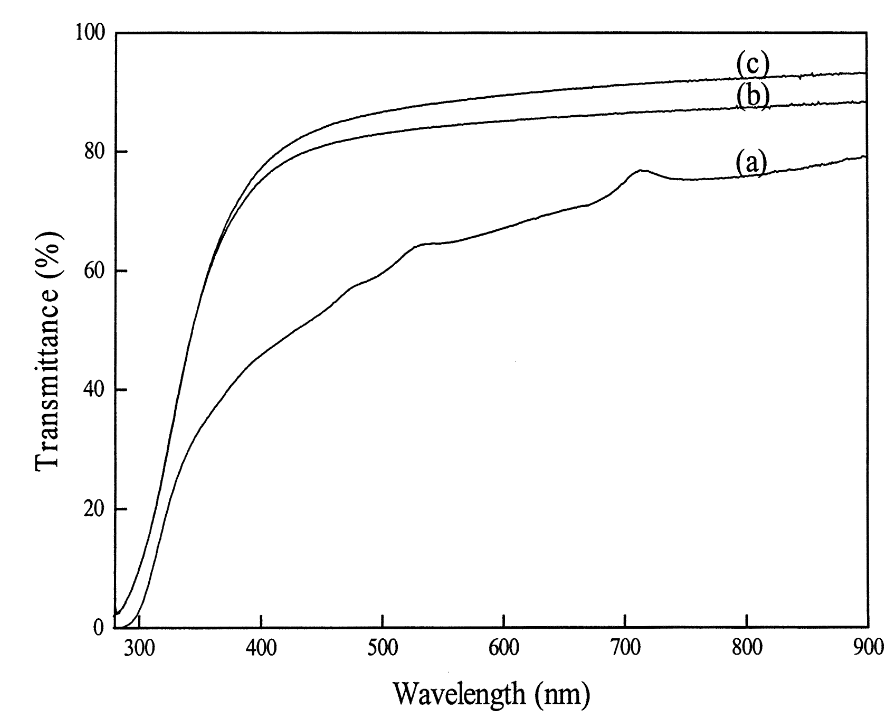
\includegraphics[width=\textwidth]{figures/Fig05b}
\end{minipage}\begin{minipage}{0.48\textwidth}
\captionof{figure}{Evolution de la transmittance de la plaque d'ITO en fonction de la longueur d'onde pour des couches de \SI{250}{\nano\meter} d'épaisseur et une température de recuit de \SI{400}{\celsius}, \SI{500}{\celsius} et \SI{600}{\celsius}}
\end{minipage}
\end{center}

\end{enumerate}
\item Caractérisations possibles : ohmmètre, brillancemètre, colorimètre et DRX.
\end{enumerate}

Les conditions optimales que l'on peut espérer avec cette procédure selon la littérature sont les suivantes : 
\begin{itemize}
\item Résistivité optimale : $\rho = 1.7 \cdot 10^{-3} ~ \si{\ohm\centi\meter}$ ;
\item Transmittance dans le visible : $> 90 ~ \si{\percent}$
\end{itemize}

\begin{comment}
\subsection{Mesure des performances électriques - \faClockO ~ \SI{1}{\hour}}

Réaliser l'acquisition des performances électriques sous DEL bleue et DEL rouge.

\begin{enumerate}
\item Test en plein soleil ou sous lampe halogène (50W)
\begin{itemize}
\item Mesurer la tension en circuit ouvert ($V_{oc}$) avec un voltmètre.
\item Mesurer le courant de court-circuit ($I_{sc}$) avec un ampèremètre.
\end{itemize}


\item Tracé de la courbe courant-potentiel :
\begin{itemize}
\item Connecter la cellule à un potentiomètre de \SI{500}{\ohm}.
\item Mesurer le courant et la tension pour différentes résistances.
\item Tracer la courbe.
\end{itemize}

\item Calcul du rendement ($\eta$) :
\begin{itemize}
\item Déterminer la puissance maximale
\item Calculer le rendement de conversion solaire pour une puissance solaire autour de \SI{1000}{\watt\per\meter\squared}.
\end{itemize}
\end{enumerate}


\section{Discussion}

\subsection{Rôle de l'électrolyte}

Dans la cellule à colorant, l'électrolyte est un mélange de triiodure/iodure et potassium. Contrairement aux cellules électrochimiques habituelles, les anions jouent un rôle dans la migration des charges, mais aussi dans le processus rédox puisqu'ils vont servire de médiateur dans le transport des électrons. 

\paragraph*{Données :}
\begin{itemize}
\item Energie de gap : rutile : \SI{3.0}{\electronvolt} ; anatase : \SI{3.2}{\electronvolt} ; 
\begin{center}
\begin{minipage}{0.48\textwidth}

\includegraphics[width=\textwidth]{figures/Fig05}
\end{minipage}\begin{minipage}{0.48\textwidth}
\captionof{figure}{Position de gap d'énergie dans le vide et au contact de l'eau}
\end{minipage}
\end{center}
\item Constante de solubilité de \ce{I2(s)} à \SI{25}{\celsius} : 
\begin{align*}
K_s (25 ~ \si{\celsius}) = 1.315 
\end{align*}
\item Potentiel rédox standard à \SI{25}{\celsius} : 
\begin{align*}
E^\circ (\ce{I2(s) / I^-(aq)}) = 0.53 ~ \si{\volt\per{ESH}}
\end{align*}
\item Constante de complexation de \ce{I2(aq)} par \ce{I^-(aq)} : 
\begin{align*}
K^\circ ( 25 ~ \si{\celsius})  \approx 723
\end{align*}

\end{itemize}


\begin{questions}


\setcounter{question}{\thefoo}

\question[2\half] En vous appuyant sur les processus rédox ayant lieu à chacune des électrodes, en déduire le sens de circulation des {\color{red} porteurs de charges.}

\begin{mybox}
\begin{solution}[5cm]

\textbf{Anode :} [\textbf{0.5}]
\begin{align*}
\ce{D^\star = D^+ + e^-}
\end{align*}

\textbf{Cathode :} [\textbf{0.5}]
\begin{align*}
\ce{I_3^-(aq) + 2e^- = 3I^-(aq)}
\end{align*}


\textbf{Equation de réaction :} [\textbf{0.5}]
\begin{align*}
\ce{2 D^\star {+} I_3^- (aq) = 2D^+(aq) + 3 I^-(aq)}
\end{align*}

\textbf{Bilan :} [\textbf{1.0}]
On trouve donc que les ions $\ce{I^-(aq)}$ sont générés à la cathode, pour être consommés par oxydation à l'anode pour régénerer les colorants $\ce{D^+}$ en $\ce{D}$. On a donc un flux d'ions \ce{I^-} du pôle $\oplus \to \ominus$.

\end{solution}
\end{mybox}

\question[4] Déterminer le potentiel rédox standard du couple \ce{I3^-(aq)/I^-(aq)} à \SI{25}{\celsius}.

\begin{mybox}
\begin{solution}[5cm]

\textbf{Demi-équation rédox} [\textbf{1.0}]
\begin{align*}
\ce{I2(s)/I^-(aq)} \quad \ce{I2(s) + 2e^- &= 2 I^- (aq)} \\
\ce{I3^-(aq)/I^-(aq)} \quad \ce{I3^-(aq) + 2e^- &= 3 I^-(aq)}
\end{align*}

\textbf{Relation entre les demi-équations rédox} [\textbf{1.5}]

\begin{align*}
\ce{I2(s) + 2e^- &= 2 I^- (aq)} \quad \Delta_{1/2} G^\circ = -2 F E^\circ (\ce{I2(s)}/\ce{I^-(aq)}) \\
\ce{I2(s) &= I2(aq)} \quad \Delta_{r} G_1^\circ = -RT \ln K_s \\
\ce{I2(aq) + I^-(aq) &= I3^-(aq)} \quad \Delta_{r} G_2^\circ = -RT \ln K^\circ
\end{align*}

En combinant judicieusement les trois réactions ci-dessus, on retrouve la demi-équation rédox associée au couple \ce{I3^-(aq)}/\ce{I^-(aq)} : [\textbf{1.0}]
\begin{align*}
\Delta_r G^\circ  ( \ce{I3^-(aq)}/\ce{I^-(aq)} ) = \Delta_{1/2} G^\circ - \Delta_r G_1^\circ - \Delta_r G_2^\circ
\end{align*}

En utilisant le fait que $\Delta_r G^\circ  ( \ce{I3^-(aq)}/\ce{I^-(aq)} ) = 2 F E^\circ (\ce{I3^-(aq)}/\ce{I^-(aq)}) $, on aboutit à :

\begin{align*}
E^\circ (\ce{I3^-(aq)}/\ce{I^-(aq)}) = E^\circ (\ce{I2(s)}/\ce{I^-(aq)}) - \frac{RT}{2F} \ln K^\circ K_s
\end{align*}

\textbf{AN} On cherche à \SI{25}{\celsius}, d'où [\textbf{0.5}]
\begin{align*}
E^\circ (\ce{I3^-(aq)}/\ce{I^-(aq)}) &= 0.53  - \frac{0.06}{2}  \log (723 \times 1.315 ) \\
&= 0.44 ~ \si{\volt\per{ESH}} 
\end{align*}

\end{solution}
\end{mybox}

\question[2] En déduire une gamme de valeur pour chacun des potentiels rédox du colorant.

\begin{mybox}
\begin{solution}[5cm]

\textbf{Axe de potentiel + plage de potentiel} [\textbf{1.0}] + [\textbf{1.0}]

\begin{center}
\begin{minipage}{0.4\textwidth}
\centering

\includegraphics[width=0.9\textwidth]{figures/Corr03}
\end{minipage}\begin{minipage}{0.56\textwidth}
\captionof{figure}{Axe de potentiel standard à \SI{25}{\celsius}}
Dans les conditions standard, on trouve alors : 
\begin{align*}
0.44 < &E^\circ (\ce{D^+}/\ce{D}) [\si{\volt\per{ESH}}] < 1.23  \\
0 < &E^\circ (\ce{D^+}/\ce{D^\star}) [\si{\volt\per{ESH}}] < 0.44
\end{align*}
\end{minipage}
\end{center}

\textbf{Nota Bene : }
\begin{enumerate}
\item En réalité, il faudrait prendre en compte les conditions réelles pour définir la gamme de potentiel rédox, ce qui conduirait probablement à une inégalité de la forme : 
\begin{align*}
E (\ce{I3^-(aq)}/\ce{I^-(aq)}) < & E (\ce{D^+}/\ce{D}) < E (\ce{O2(g)}/\ce{H2O(l)})  \\
\max \left\{ E (\ce{H^+(aq)}/\ce{H2(g)}) ; E (\ce{TiO2}/\ce{TiO2^-}) \right\} < & E (\ce{D^+}/\ce{D^\star}) < E (\ce{I3^-(aq)}/\ce{I^-(aq)})
\end{align*}
Mais on manque d'information pour prendre en compte l'écart aux conditions standard.
\item Il faudrait probablement prendre en compte que \ce{TiO2} n'est pas forcément de l'anatase à \SI{100}{\percent}, mais qu'il s'agit d'un mélange.
\end{enumerate}

\end{solution}
\end{mybox}

\setcounter{foo}{\value{question}}
\end{questions}

\subsection{Rôle du colorant}

Les anthocyanes sont des pigments naturels appartenant à la famille de sflavonoïdes, largement présents dans les végétaux. Ils sont responsables des couleurs rouges, bleues et violettes abservées dans les fleurs, fruits, $\ldots$ \`{A} cela s'ajoute des propriétés anti-oxydantes et anti-inflammatoires qui les rendent bénéfiques pour la santé humaine, expliquant leur utilisant de plus en plus courante aux colorants artificiels dans l'industrie agroalimentaire et cosmétique.

\begin{center}
\begin{minipage}{0.48\textwidth}
\centering
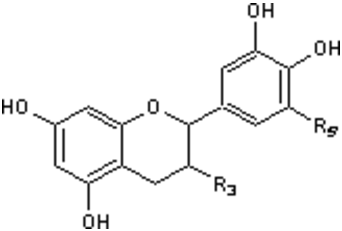
\includegraphics[width=0.5\textwidth]{figures/Fig04.pdf}
\end{minipage}\begin{minipage}{0.48\textwidth}
\captionof{figure}{Structures de la famille des anthocyanes où les positions $3'$ et $5'$ peuvent être substituées de manière variable.}
\end{minipage}
\end{center}%https://tice.ac-montpellier.fr/ABCDORGA/Famille/FLAVONOIDES.html

\begin{questions}
\setcounter{question}{\thefoo}

\question[2] Quelle transition électronique est mis-en-jeux dans ces composés ? Quels paramètres influencent l'énergie de la transition électronique ?%pH, substitution

\begin{mybox}
\begin{solution}[5cm]

Molécule fortement conjuguée, ce qui permet des transitions électroniques $\pi \to \pi^\star$ dans le domaine du visibile. [\textbf{1.0}]

Les transitions électroniques peuvent être influencées par les effets de milieu : solvant, $pH$, température$\ldots$  [\textbf{1.0}]


\end{solution}
\end{mybox}

\question[3] Réaliser le spectre UV-Visible d'un jus d'anthocyane. En déduire la longueur d'onde et l'énergie de la transition électronique dans le visible. En quoi cette transition est-elle complémentaire au pigment \ce{TiO2} ? Le panneau aurait-il pu fonctionner sans le colorant ?

\begin{mybox}
\begin{solution}[5cm]

Si on assume que seul les anthocyanes absorbent dans le jus de framboise, on on trouve deux maximums : un autour de \SI{310}{\nano\meter} et l'autre autour de \SI{520}{\nano\meter}. [\textbf{0.5}]

On peut en déduire l'existence de deux transitions électroniques dans le visible : [\textbf{0.5}]

\begin{align*}
\lambda_1 = 310 ~ \si{\nano\meter} &\iff \Delta E_1 \approx \SI{4.0}{\electronvolt} \\
\lambda_2 = 520 ~ \si{\nano\meter} &\iff \Delta E_2 \approx \SI{2.4}{\electronvolt}
\end{align*}

Cette transition est complémentaire au \ce{TiO2} car on observe une absorption non nulle sur une grande partie du spectre visible, ce qui permet de capter la grande majorité des photons de la lumière solaire. [\textbf{1.0}]

Le fonctionnement du panneau dépendrait de la source. Ici, le panneau ne fonctionnerait pas avec nos sources lumineuses (DEL) monochromatiques dans le visible. Par contre, il capterait probablement les photons UV proche émis par le soleil. Cependant, il ne faudrat pas s'attendre à un rendement très important. [\textbf{1.0}]



\end{solution}
\end{mybox}

\question[3] Illustrer l'adsorption chimique des anthocyanes à la surface du dioxyde de titane.

\begin{mybox}
\begin{solution}[5cm]

Il semble assez intuitif que les anthocyanes puissent se chimisorber spontanément sur \ce{TiO2} facilitant le transfert d'électron du colorant vers le semi-conducteur. [\textbf{1.0}]

Le groupement catéchol semble être l'ensemble fonctionnel le plus à même de se condenser au contact d'une surface d'anatase. [\textbf{1.0}]

\textbf{Schéma de l'adsorption :} [\textbf{1.0}]

\begin{center}

\includegraphics[width=0.4\textwidth]{figures/Corr04}
\end{center}

\end{solution}
\end{mybox}

\question[0] {\color{red} A l'aide d'un microscope optique, réaliser un schéma de votre observation microscopique. Commenter l'uniformité de l'adsorption du colorant sur la surface. Que peut-on observé au niveau de la surface de \ce{TiO2} ? Quel en est l'origine ?}

\begin{mybox}
\begin{solution}[5cm]

Non traité cette année. A voir si on voit qqc d'intéressant.

\end{solution}
\end{mybox}

\question[1] Les propriétés d'absorption et d'adsorption sont-elles suffisantes pour obtenir un photocourant ? Quelle autre propriété physico-chimique doit faire parti du cahier des charges minimal d'un colorant ?

\begin{mybox}
\begin{solution}[5cm]

Capacité à transférer ses électrons vers l'électrode. Au cahier des charges, il faut ajouter les propriétés rédox.

\end{solution}
\end{mybox}

\setcounter{foo}{\value{question}}
\end{questions}


\subsection{Performance de votre cellule solaire}



\begin{questions}
\setcounter{question}{\thefoo}
\question[2] Faites l'acquisition de la caractéristique, en convention récepteur, de votre cellule solaire. Vous penserez à annoter précisément les paramètres expérimentaux de votre acquisition.

\begin{mybox}
\begin{solution}[5cm]

\`{A} faire

\end{solution}
\end{mybox}

\question[1] En déduire l'évolution de la puissance reçue par votre cellule solaire en fonction de la tension.

\begin{mybox}
\begin{solution}[5cm]

\`{A} faire

\end{solution}
\end{mybox}

\question[3] Déterminer les paramètres expérimentaux de votre cellule en justifiant votre manière de procéder : 

\begin{center}
\begin{tabular}{C{2cm}C{2cm}C{2cm}C{2cm}C{2cm}C{2cm}C{2cm}}
\toprule
& $U_{max} ~ [\si{\volt}]$ & $I_{max} ~ [\si{\milli\ampere}]$ & $U_{oc} ~ [\si{\volt}]$ & $I_{cc} ~ [\si{\milli\ampere}]$ & $FF$ & $r_{max}$ \\
\midrule

DEL rouge & & & & & & \\
DEL bleue & & & & & & \\
\bottomrule
\end{tabular}
\end{center}

\begin{mybox}
\begin{solution}[5cm]

\`{A} faire

\end{solution}
\end{mybox}

%\question[1] lala
\setcounter{foo}{\value{question}}
\end{questions} 


\newpage

\section*{Barème}

\begin{minipage}{0.33\textwidth}
Noms-Prénoms du binôme
\end{minipage}\begin{minipage}{0.33\textwidth}
$n^\circ 1$ :
\end{minipage}\begin{minipage}{0.33\textwidth}
$n^\circ 2$ :
\end{minipage}

\begin{questions}
\setcounter{question}{\thefoo}

\titledquestion{Cahier de laboratoire}[4] Tenue du cahier de laboratoire.

%\titledquestion{Investissement}[2] Variable d'ajustement à la liberté du correcteur en fonction de l'investissement, de la qualité des raisonnements et de la démarche d'investigation du binôme.

\end{questions}

\begin{center}
\gradetable
%\bonusgradetable
\end{center}

\end{comment}

\end{document}
